\documentclass[12pt]{article}

\usepackage[margin=1.0in]{geometry}
\usepackage{color}
\usepackage{times}
\usepackage[pdftex]{hyperref}

\newcommand{\fillin}[1]{\textcolor{red}{\textsc{#1}}}

\pagestyle{empty}
\setlength{\parindent}{0in}
\setlength{\parskip}{2ex}
\renewcommand{\baselinestretch}{1.0}

\usepackage{graphicx}
\usepackage{caption}
\usepackage{float}

\begin{document}

\begin{title}
	{\Large\bf Homework 1, Math 455: Due Monday, 01/22/2018}
\end{title}

\author{\bf Alexander Van Roijen}

\maketitle
{\bf Instructions}:  The homework assignment editing this \LaTeX\ document.  Download the \LaTeX\ source from the class web page and study
it to learn more about \LaTeX.  Replace the text with appropriate information.  Run ``pdflatex'' on this document.

You will submit this assignment in two parts:
\begin{enumerate}
\item Print out the PDF file and bring it to class, and
\item Send an e-mail to:
\begin{center}
gang@math.binghamton.edu
\end{center}
\emph{before class} on the due date with two attachments:
\begin{itemize}
\item The \LaTeX\ source file, and
\item The generated PDF document.
\end{itemize}
\end{enumerate}

Please complete the following:
\begin{enumerate}
\item ``Paste'' a photograph of you below using a \LaTeX\ float.  Write your name in the caption and a sentence about something that makes you unique.  (See Tutorial XI in \href{https://www.tug.org/twg/mactex/tutorials/ltxprimer-1.0.pdf}{\LaTeX\ Tutorials: A Primer}.) \\

\begin{figure}[H]
\centering
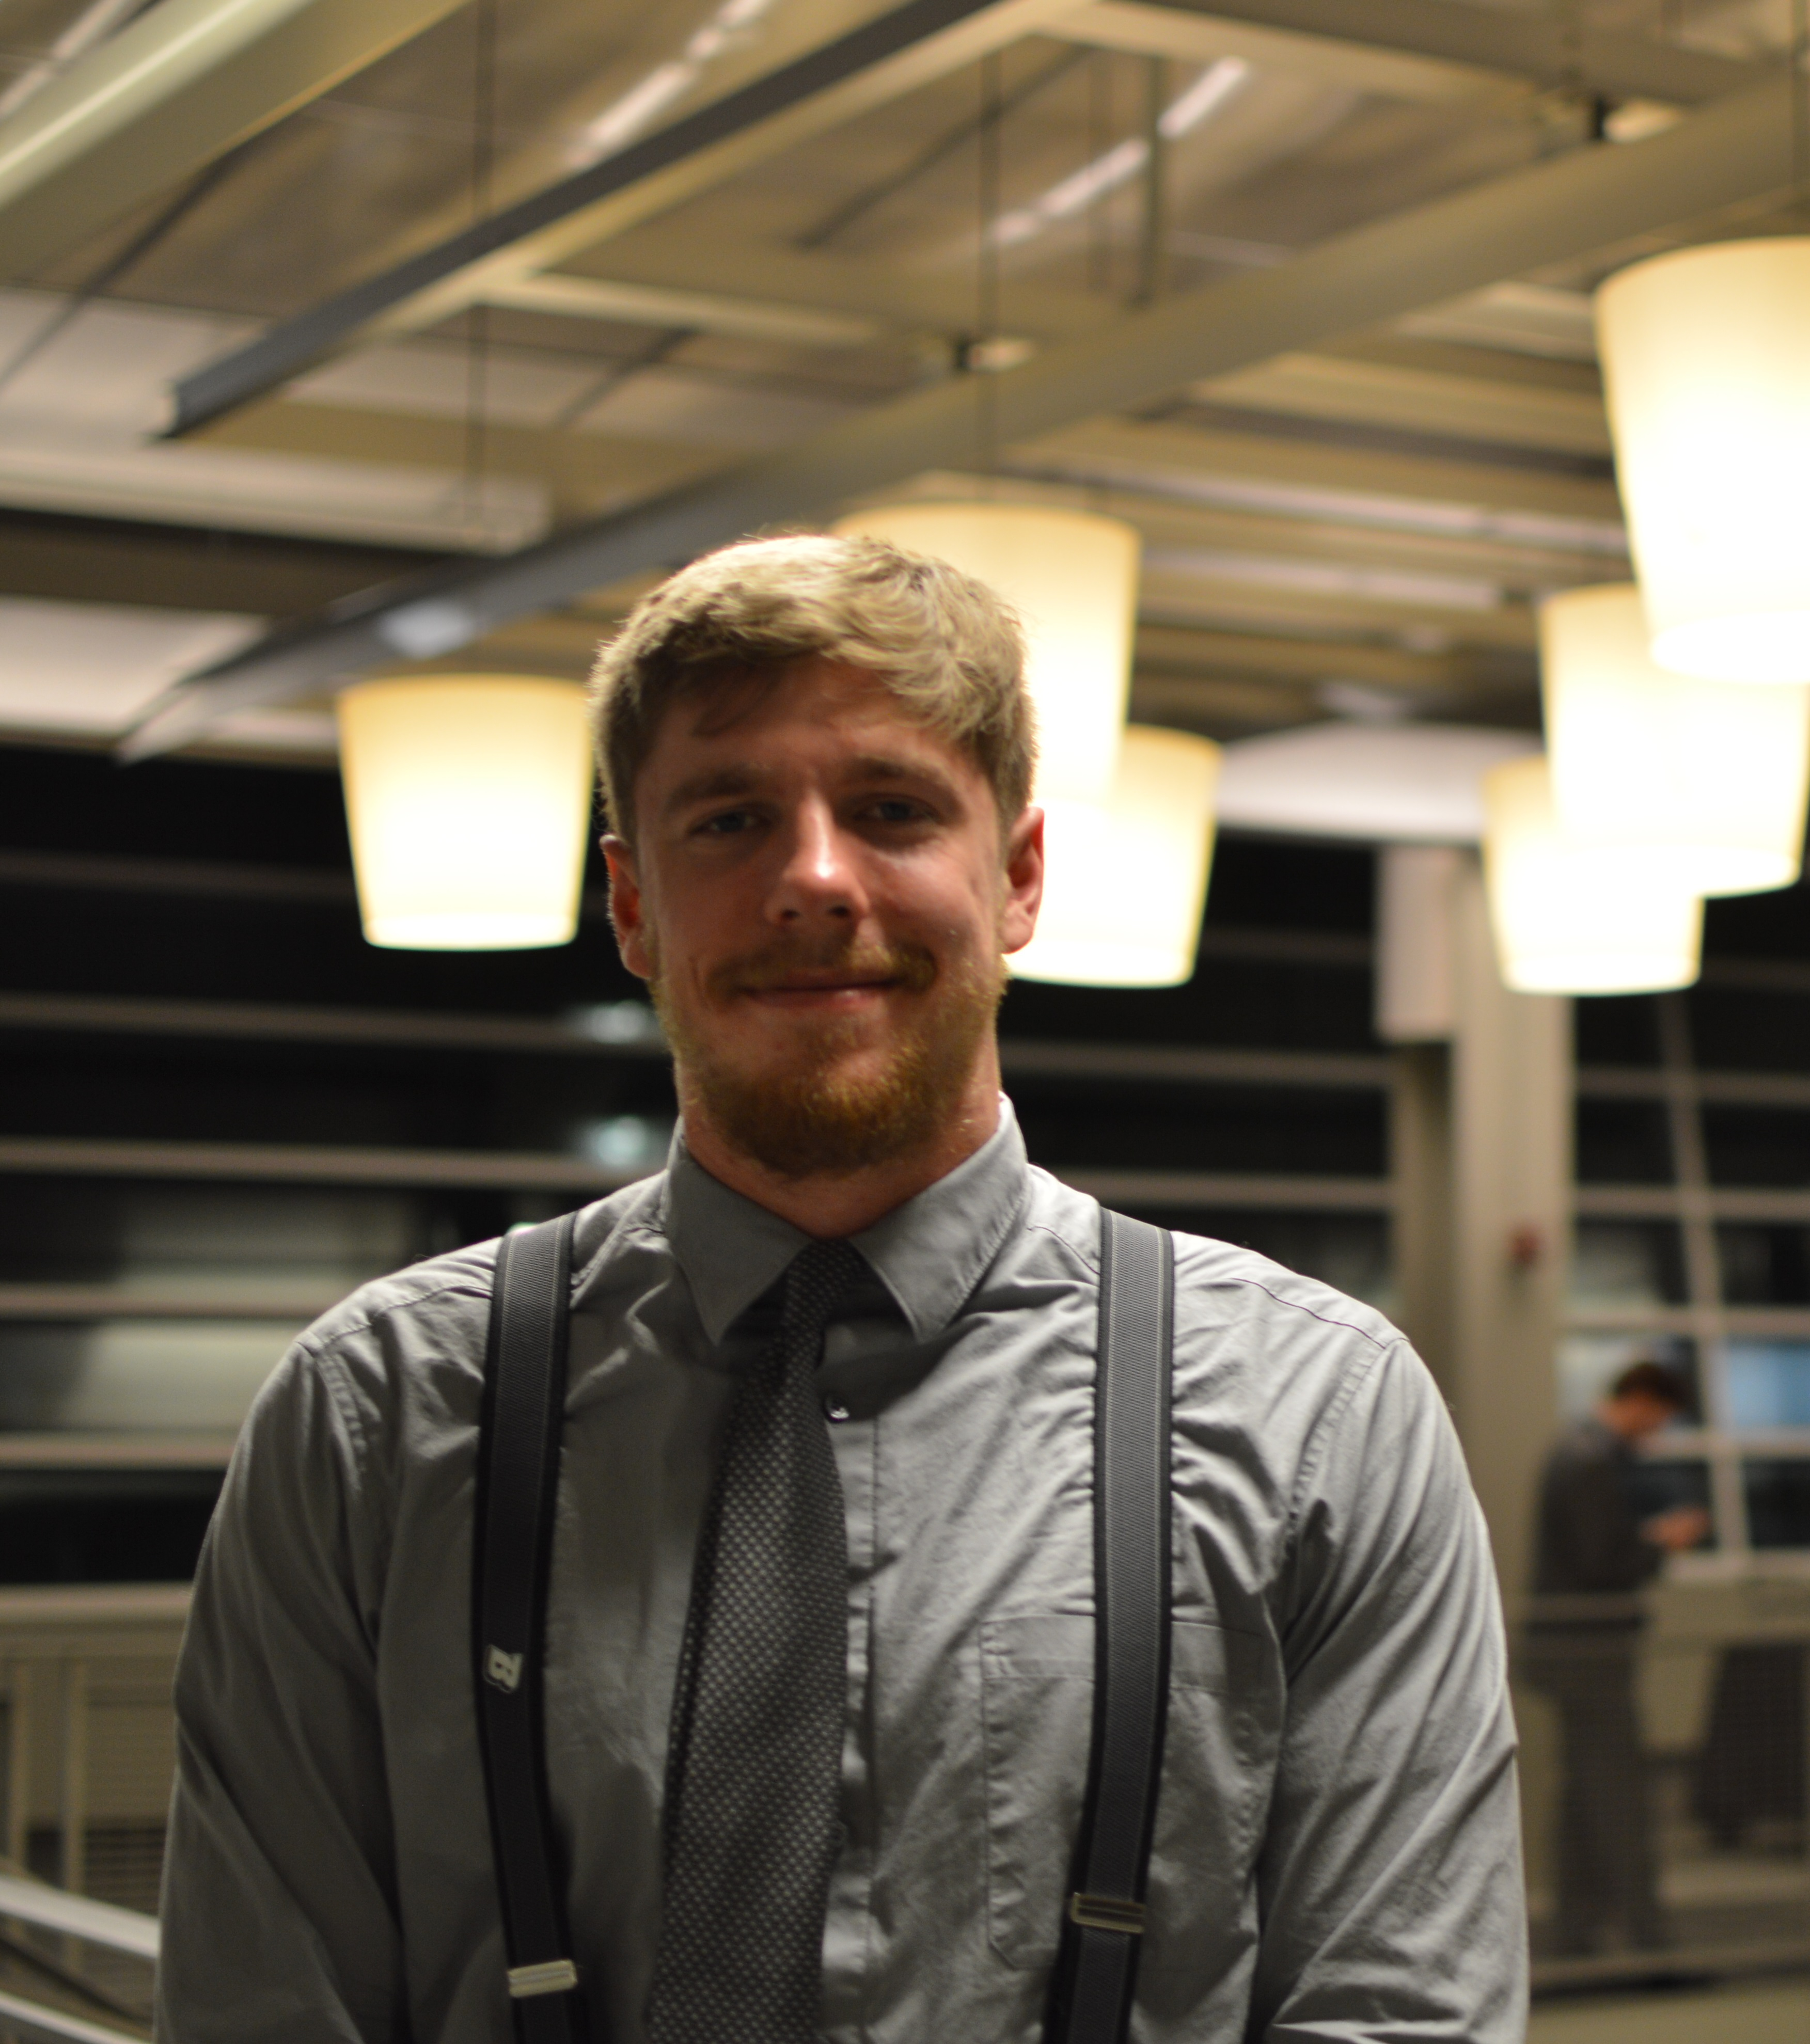
\includegraphics[width=10cm,height=10cm]{cropped.jpg}
\caption[Alexander Van Roijen]{Alexander Van Roijen: \\I can dunk a basketball sometimes; im working on it.}
\label{alexV}
\end{figure}

\item What state or country are you from?  How is your name pronounced?\\
\fillin{Originally from the Netherlands; moved to New York when I was 5. My name is pronounced Al-x-and-er Van Roy-en}
\item Is your ultimate intention to obtain an undergraduate degree, a master's degree or a Ph.D.?\\
\fillin{No idea! Currently undergraduate, i am applying to masters programs as well as jobs, hope to be doing something awesome though!}
\item What was your major as an undergraduate?\\
\fillin{Mathematics and Computer Science, Dual Degree}
\item How many statistics classes have you taken at the undergraduate level?  How many at the graduate level?\\
\fillin{2? Mainly Math 448, but also CS 448: Machine Learning}
\item Have you ever used Linux or UNIX before?  If so, describe the nature of your exposure.
\fillin{As a C.S. major, we are constantly using linux. I feel very comfortable with it. I have also used it for my own solo projects and at my internships}
\item What programming languages, if any, have you been exposed to?  How many classes have you taken in each of these languages?  How many years experience do you have with each of them?\\
\fillin{R, Python, Java, C++, C, Perl,  JavaScript, C\#, Haskell, Ruby. I took classes in C, C++, Java, and Haskell. I have had 2 years working with Python, 3 years with Java, 3 years with C/C++, 1 semester with R}
\item In late 1905, Albert Einstein published "Does the Inertia of a Body Depend Upon Its Energy Content?" which introduced the now famous equation that the energy of a body at rest (E) equals its mass (m) times the speed of light (c) squared.  Write this formula as a \LaTeX\ equation.\\
\fillin{$E=mc^2$}
%This line and the next is "commented out".
%\item Find a photograph on the Internet of a prominent statistician.  ``Paste'' the picture below using a \LaTeX\ float.  Write his/her name in the caption and a sentance about his/her notable contribution to statistics.  (Hint 1:  The \href{http://wikipedia.org}{Wikipedia} website is a great resource.  Hint 2:  See Tutorial XI in \href{http://www.stat.tamu.edu/~dahl/teaching/604/lecture/l02/ltxprimer.pdf}{\LaTeX\ Tutorials: A Primer}.)\\
\end{enumerate}

\end{document}
